\documentclass{beamer}
\usetheme{Copenhagen}
\setbeamertemplate{caption}[numbered]

\graphicspath{ {./images/} }
\usepackage{grffile}

\usepackage{hyperref}
\usepackage{tikz}
\usepackage[siunitx]{circuitikz}
\usepackage{siunitx}

\title{Characterisation of the Copenhagen Board}
\subtitle{End of Project Presentation}
\institute{SQA Summer Research Scholarship}
\author{Cory Aitchison}
\date{Summer 2021}

\begin{document}

\begin{frame}
    \titlepage
\end{frame}

\section{Introduction}

\subsection{Aims}

\begin{frame}
    \frametitle{Outline}
    \begin{columns}
        \begin{column}{0.3\textwidth}
            \tableofcontents
        \end{column}
        \begin{column}{0.6\textwidth}
            \begin{description}
                \item[Aim] $\bullet$ To characterise the RF operation of the Copenhagen board
                \item[] $\bullet$ To perform RF reflectometry on a transistor connected to the board
                \item[] $\bullet$ To optimise the resonance circuit for resistance matching
            \end{description}
        \end{column}
    \end{columns}
\end{frame}

\subsection{Equipment}

\begin{frame}
    \frametitle{Copenhagen Board}

    \begin{columns}
        \begin{column}{0.5\textwidth}
            The Copenhagen Board (CPH) allows for connections to a device via both DC and high-frequency circuitry, with spaces for additions of resistors, capacitors, and inductors.

            \begin{itemize}
                \item Manufactured by QDEV
                \item Specially designed for quantum devices
                \item 50 DC lines
                \item 16 AC lines (up to $18 \si{\giga\hertz}$)
                \item 4 multiplexed LC tank circuits
            \end{itemize}



        \end{column}
        \begin{column}{0.5\textwidth}
            \begin{figure}
                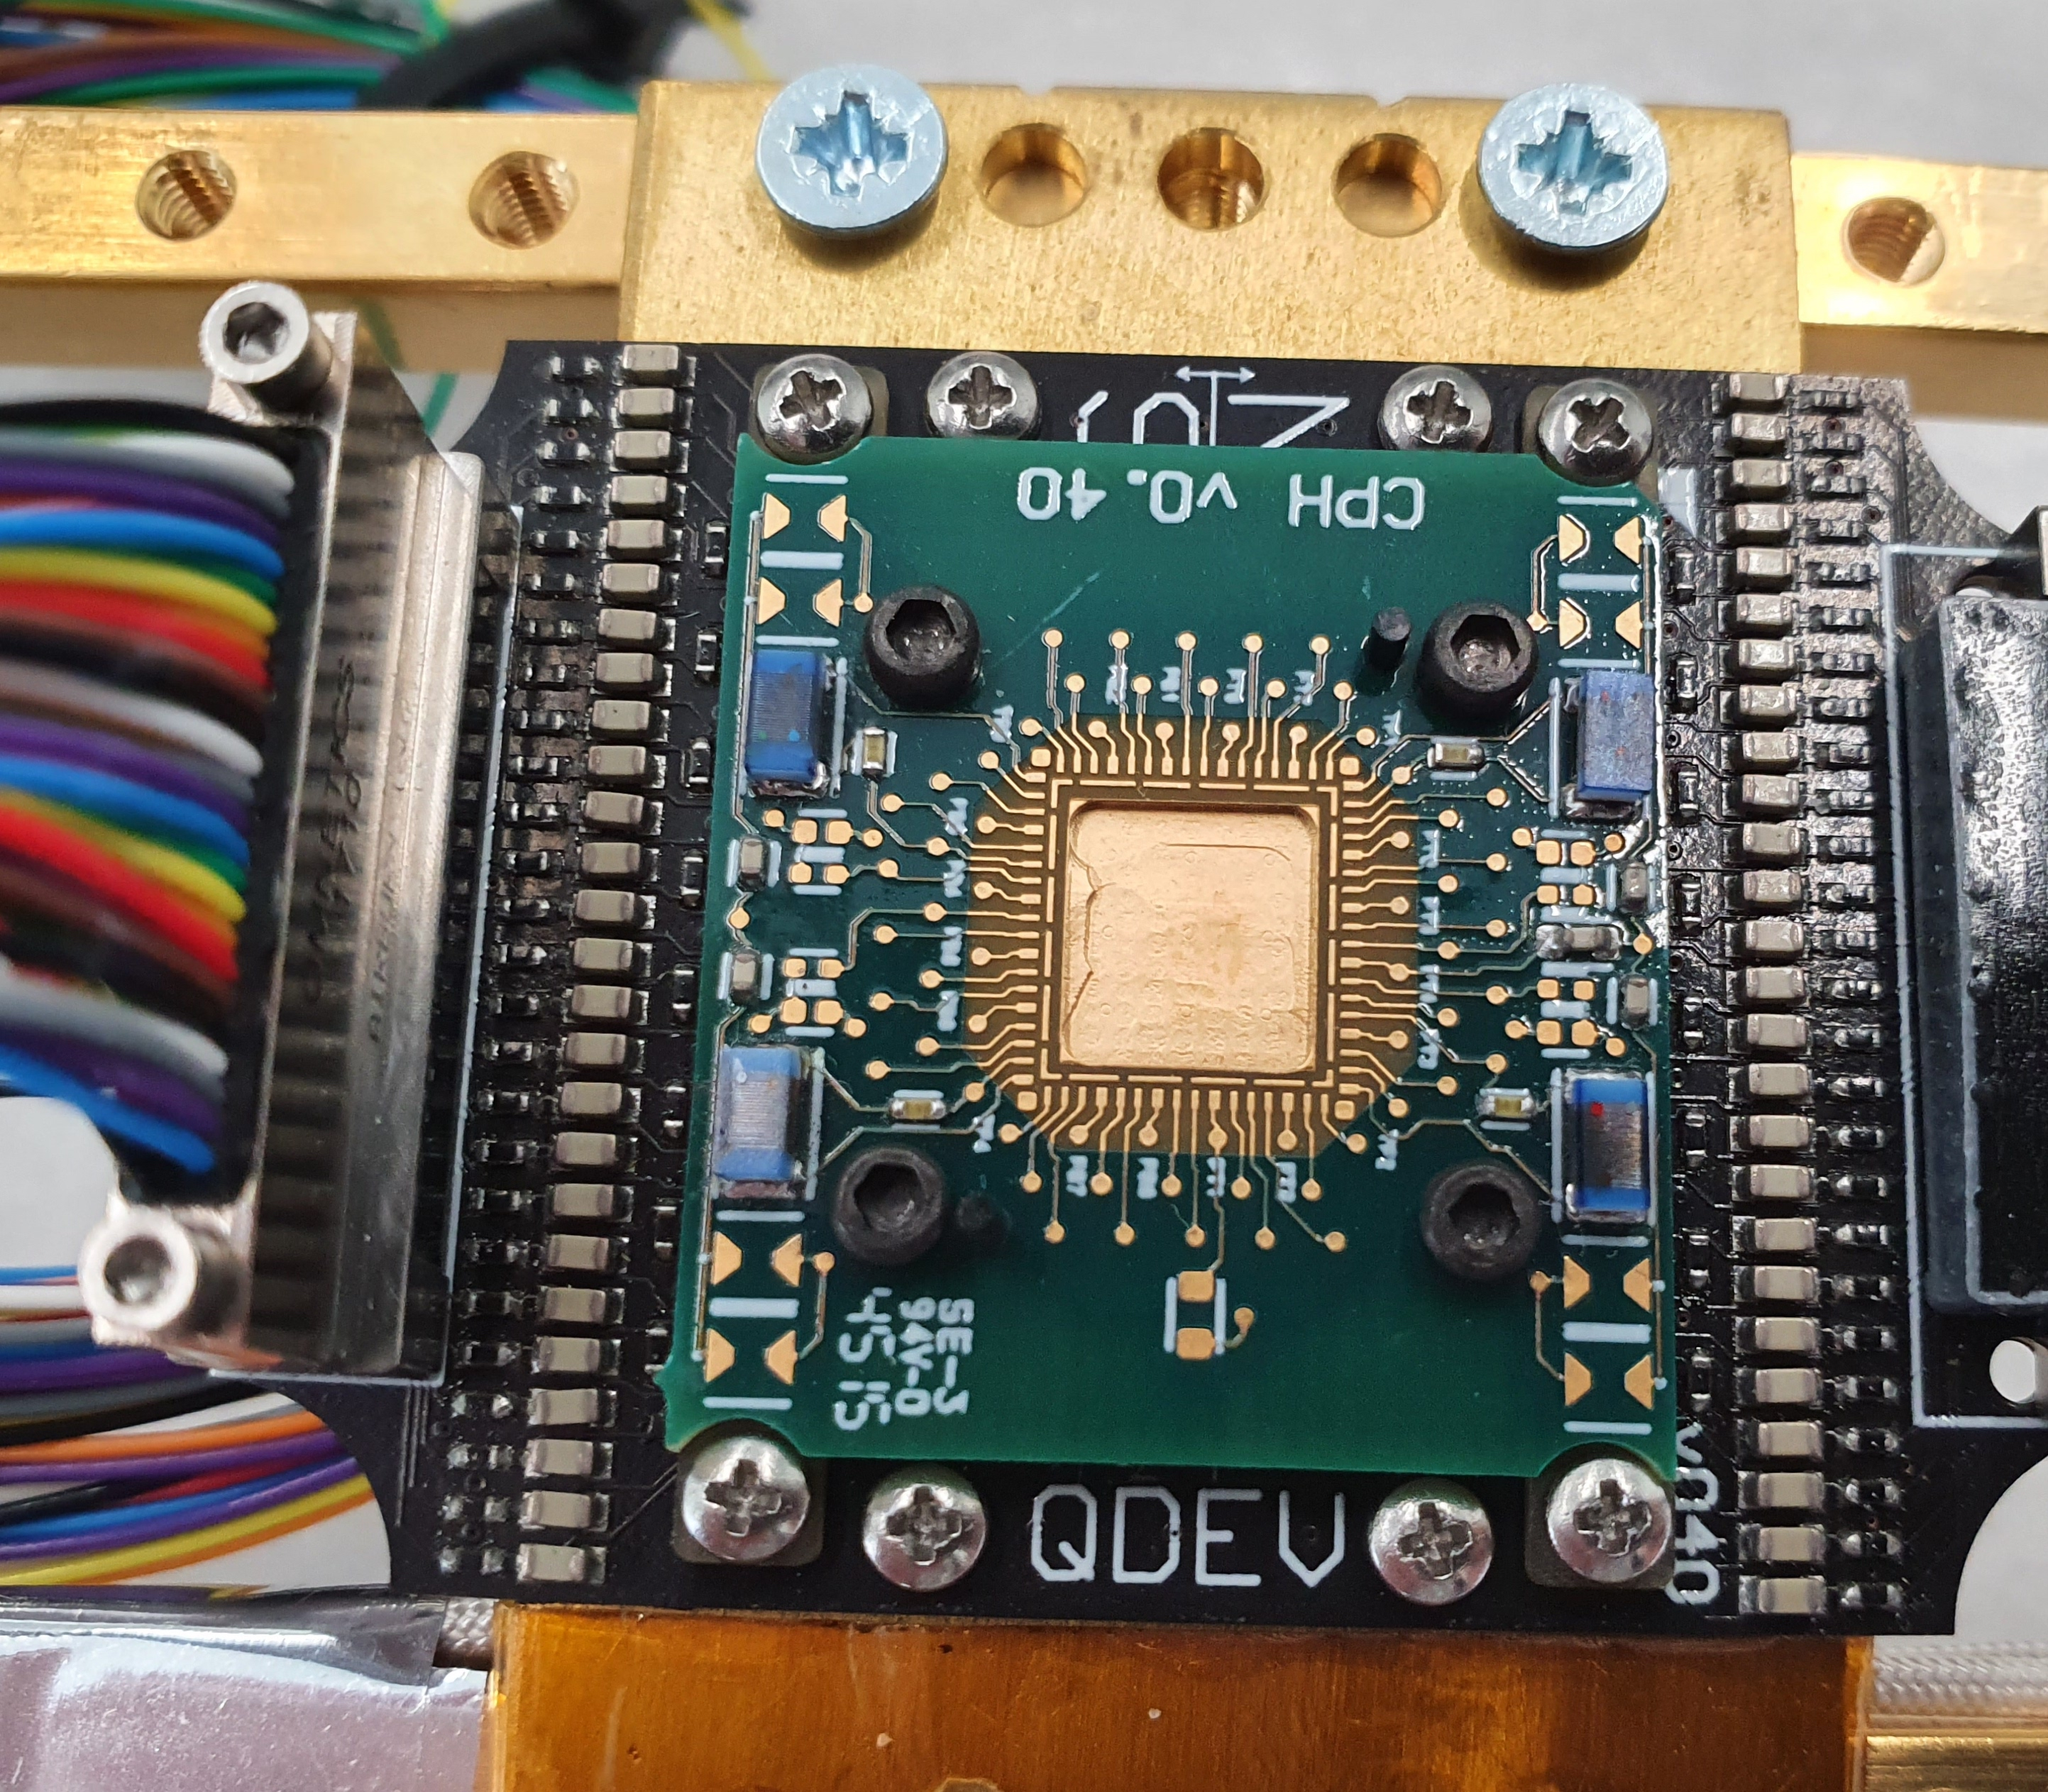
\includegraphics[width=\textwidth]{cphboard.jpg}
                \caption{Copenhagen motherboard (black) and daughter board (green).}
                \label{fig:cphboard}
            \end{figure}
        \end{column}
    \end{columns}
\end{frame}

\begin{frame}
    \frametitle{Copenhagen Board}

    \begin{itemize}
        \item Although CPH has been used for DC measurements, its usage under RF AC measurements is unfamiliar
        \item RF measurements can be beneficial because they allow for larger bandwidth (faster timescales) and lower $1/f$ noise
        \item Characterisation of the board involves understanding its circuitry, resonance, and the role of the inductors, capacitors, and resistors
    \end{itemize}

\end{frame}

\begin{frame}
    \frametitle{MOSFET Transistor}

    \begin{columns}
        \begin{column}{0.5\textwidth}
            \begin{itemize}
                \item To characterise the CPH board, a transistor can be used as a placeholder for more complex quantum devices
                \item The transistor is a MOSFET - a \emph{metal oxide semiconductor field-effect transistor}
            \end{itemize}
        \end{column}
        \begin{column}{0.5\textwidth}
            \begin{figure}
                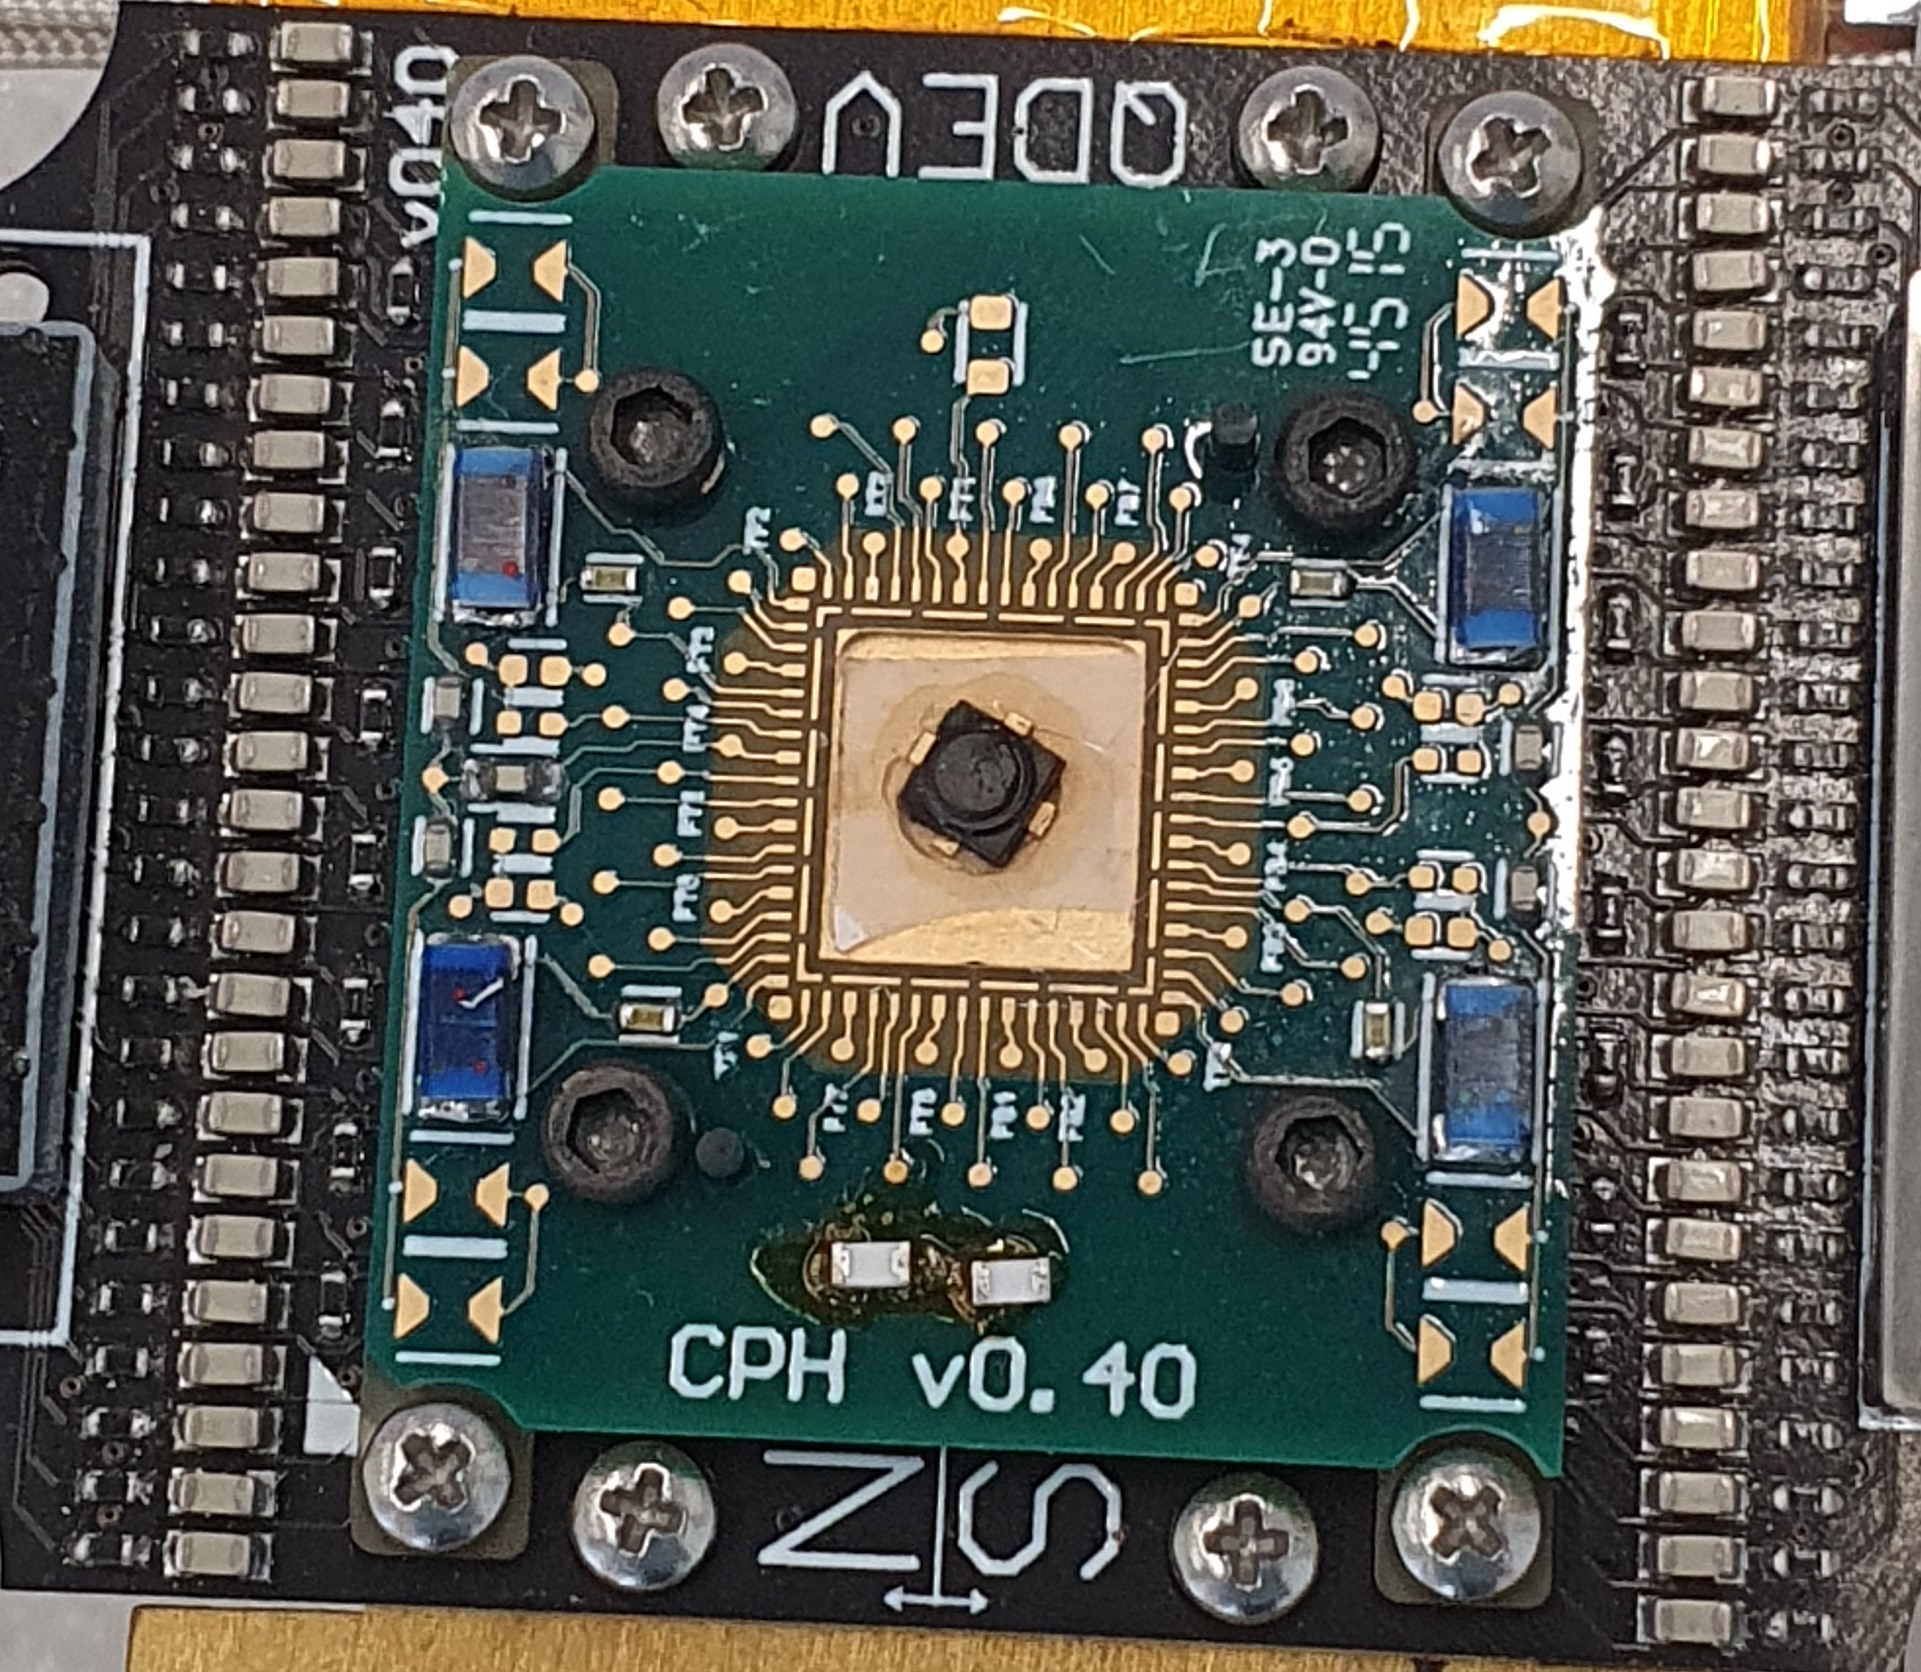
\includegraphics[width=\textwidth]{cphboardtrans.jpg}
                \caption{Transistor (black square in the gold) bonded to the daughter board.}
                \label{fig:cphboardtrans}
            \end{figure}
        \end{column}
    \end{columns}

\end{frame}

\section{Characterisation}

\subsection{Operation}

\begin{frame}
    \frametitle{Transistor Characterisation}

    \begin{columns}
        \begin{column}{0.5\textwidth}
            \begin{itemize}
                \item First need to determine if the transistor is operating correctly
                \item 4-wire sensing was used to isolate the resistance of the transistor
                \item The CPH board included $\sim 7.4\si{\kilo\ohm}$ resistors in series
            \end{itemize}
        \end{column}
        \begin{column}{0.5\textwidth}
            \begin{figure}
                \begin{circuitikz}
                    \draw
                    (0,0) to[short, o-, i=$I$] (1,0) to[R, l=$R_1$] (2.5,0) to[R, l=$R_2$] (2.5,-2) to[R, l=$R_3$] (1,-2) to[short, -o] (0,-2)
                    (2.5,0) to[short, *-] ++(1.5,0) to[rmeter, t=V, l=$v_\mathrm{4-term}$] ++(0, -2) to[short, -*] ++(-1.5, 0);
                \end{circuitikz}
                \caption{4-wire resistance sensing to determine $R_2 = v_\mathrm{4-term}/I$.}
                \label{fig:4wirecircuit}
            \end{figure}
        \end{column}
    \end{columns}
\end{frame}

\begin{frame}
    \frametitle{Results - 4-wire Sensing}

    \begin{figure}
        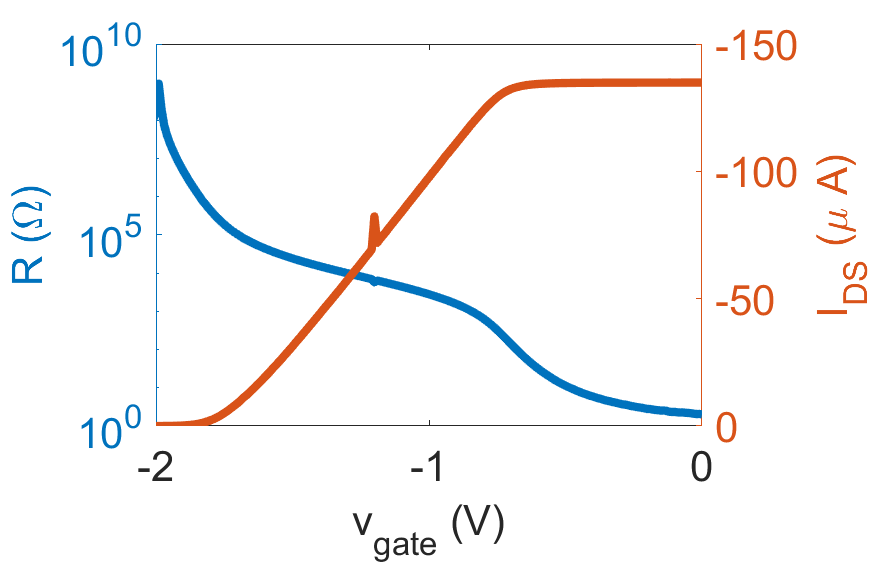
\includegraphics[width = 0.75\textwidth]{matlab_current_line.png}
        \caption{Current and resistance of the transistor as a function of gate voltage. Drain-source voltage is held constant at $v_{DS} = -1\si{\volt}$.}
        \label{fig:4wirecurrentline}
    \end{figure}

\end{frame}

\begin{frame}
    \frametitle{Results - 4-wire Sensing}

    \begin{columns}
        \begin{column}{0.5\textwidth}
            \begin{figure}
                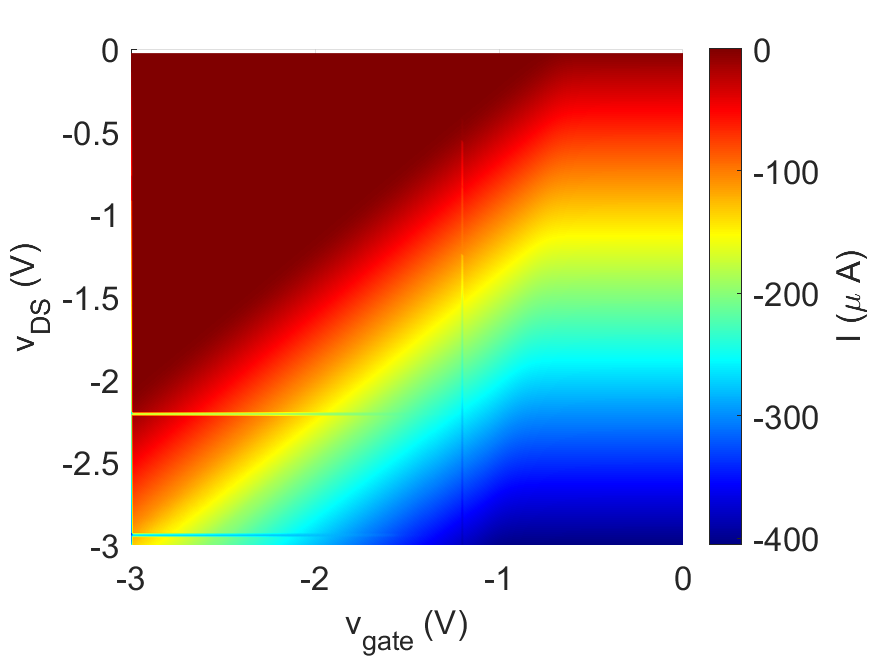
\includegraphics[width = 1.1\textwidth]{210208resistance_005_2021.02.10.17.23.31_final_i.png}
                \caption{Current through the transistor as a map of drain-source and gate voltages.}
                \label{fig:4wirecurrent}
            \end{figure}
        \end{column}
        \begin{column}{0.5\textwidth}
            \begin{figure}
                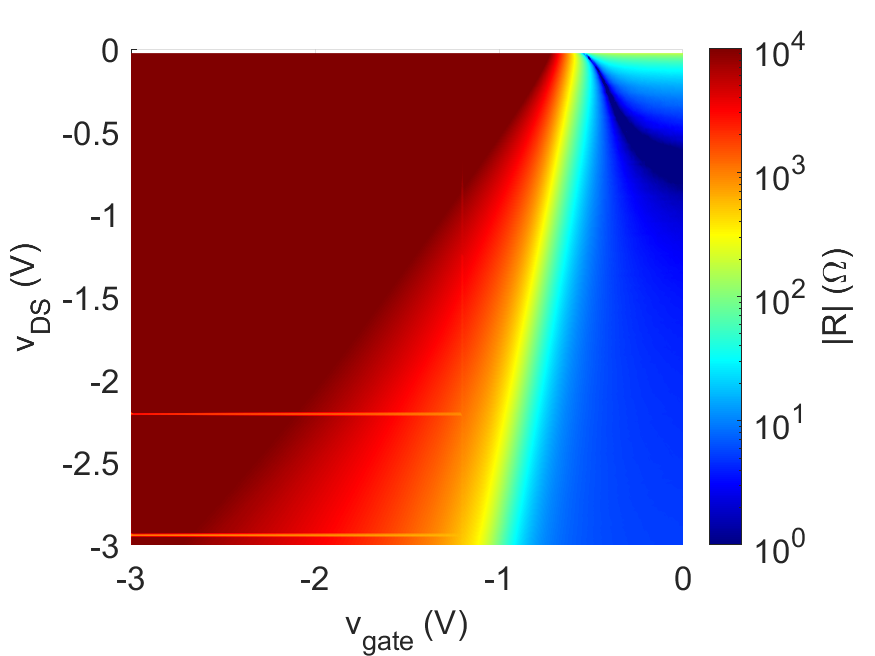
\includegraphics[width = 1.1\textwidth]{210208resistance_005_2021.02.10.17.23.31_final_res.png}
                \caption{Resistance of the transistor, using 4-wire sensing}
                \label{fig:4wireresistance}
            \end{figure}
        \end{column}
    \end{columns}

\end{frame}

\subsection{Reflectometry}

\begin{frame}
    \frametitle{RF Reflectometry}

    \begin{columns}
        \begin{column}{0.5\textwidth}
            \begin{itemize}
                \item Reflectometry allows us to probe the resistance of the transistor
                \item RF signals are inputted and reflected power is given by the following:
            \end{itemize}
            \begin{align}
                Z_t    & = i\omega L + \frac1{\frac1R + i\omega C_p} \\
                \Gamma & = \frac{Z_t - Z_0}{Z_t + Z_0}               \\
                S11    & = |\Gamma|^2
                \label{eq:s11}
            \end{align}
        \end{column}
        \begin{column}{0.5\textwidth}

            \begin{figure}
                \centering
                \begin{circuitikz}[scale = 0.8] \draw
                    (0,0) to[short, o-, i=$~$] (0,-1) to[inductor, l_=$L$, -*] (0,-3)
                    (-1,-3) -- (1, -3) to[capacitor, l=$C_p$] (1, -5) -- (-1,-5) to[vR, l=$R$] (-1,-3)
                    (0, -5) to[short, *-] (0, -5.2) node[ground]{};
                \end{circuitikz}
                \caption{RLC circuit for RF reflectometry.}
                \label{fig:og_circuit}
            \end{figure}

        \end{column}
    \end{columns}

\end{frame}

\begin{frame}
    \frametitle{RF Reflectometry}

    An inital RF-sweep without bonds to the transistor shows resonant peaks at frequencies corresponding to the four inductors:

    \begin{table}[htp]
        \centering
        \begin{tabular}{| c | c  | c | c | c |}
            \hline
            Inductor & $f_\mathrm{res}$ (\si{\mega\hertz}) & $L$ (\si{\nano\henry}) & $C_p$ (\si{\pico\farad}) & Status \\[0.5ex]
            \hline \hline
            $L1$     & $164$                               & $1200$                 & $0.79$                   & -      \\
            $L2$     & $192$                               & $820$                  & $0.84$                   & -      \\
            $L3$     & $186$                               & $560$                  & $1.3$                    & Gate   \\
            $L4$     & $50$                                & $390$                  & $26$                     & Source \\ \hline
        \end{tabular}
        \caption{Measured resonant frequencies for each inductor on the Copenhagen board; Parasitic capacitance calculated using $f_\mathrm{res} = 1/2\pi\sqrt{LC_p}$.}
        \label{table:capacitances}
    \end{table}

\end{frame}

\begin{frame}
    %% Resonance is not at 50 MHz because we are looking at (Z-50)/(Z+50) not just minimising Im(Z)

    \frametitle{RF Reflectometry Simulations}
    Using $L = 390 \si{\nano\henry}$, $C_p = 26\si{\pico\farad}$, we simulate theoretical reflectance using Equation \ref{eq:s11}:
    \begin{columns}
        \begin{column}{0.5\textwidth}
            \begin{figure}
                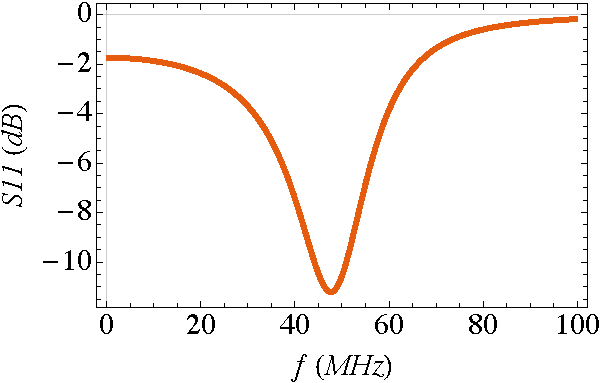
\includegraphics[width=\textwidth]{S11_resonance.pdf}
                \caption{Simulated resonance peak at $R=1\si{\kilo\ohm}$ and $C_p = 26\si{\pico\farad}$. Resonance occurs at $f \approx 48\si{\mega\hertz}$.}
                \label{fig:resonancesim}
            \end{figure}
        \end{column}
        \begin{column}{0.5\textwidth}
            \begin{figure}
                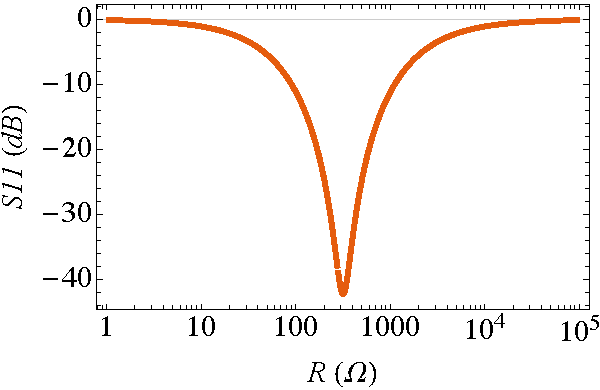
\includegraphics[width = \textwidth]{S11_cs0db.pdf}
                \caption{Simulated transfer function at resonant frequency.}
                \label{fig:s11cs0db}
            \end{figure}
        \end{column}
    \end{columns}


\end{frame}

\begin{frame}
    \frametitle{RF Reflectometry Measurements}

    \begin{columns}
        \begin{column}{0.5\textwidth}
            \begin{figure}
                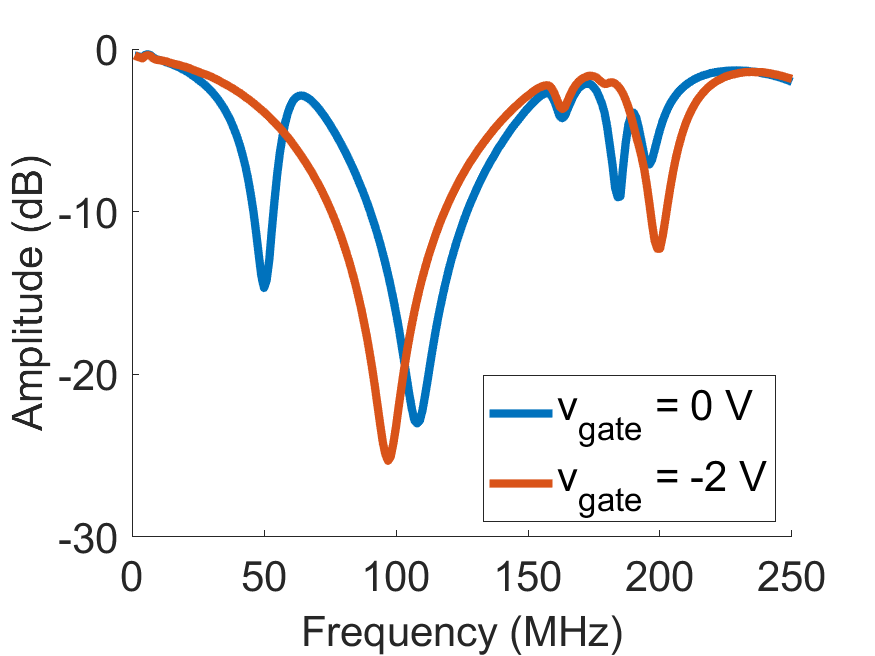
\includegraphics[width = 1.1\textwidth]{matlab_cs0_resonance.png}
                \caption{Resonance peaks at different gate voltages.}
                \label{fig:cs0res}
            \end{figure}
        \end{column}
        \begin{column}{0.5\textwidth}
            \begin{figure}
                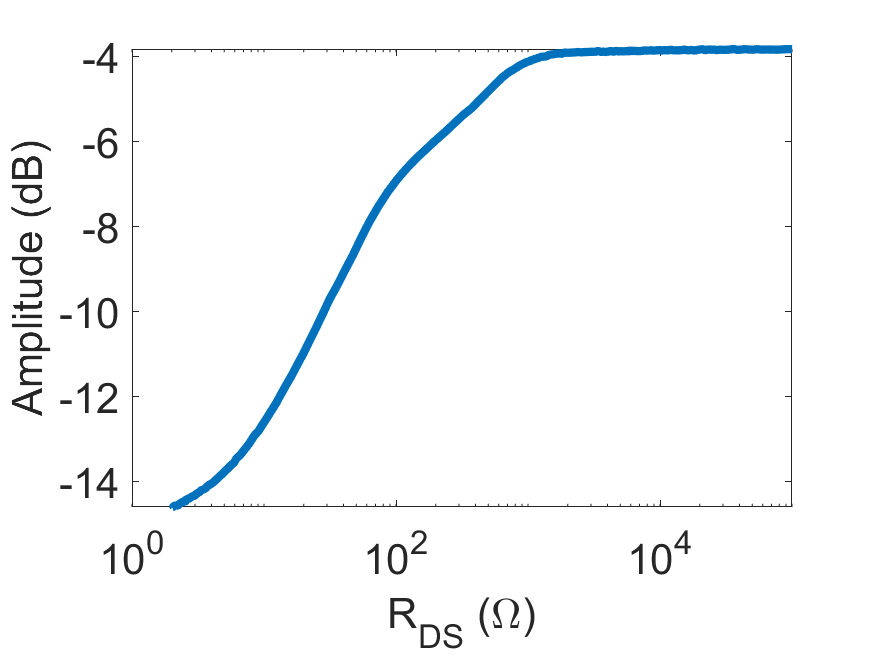
\includegraphics[width = 1.1\textwidth]{matlab_cs0_transfer.png}
                \caption{Transfer function at $f = 50\si{\mega\hertz}$ and $v_{DS} = -1\si{\volt}$.}
                \label{fig:cs0transfer}
            \end{figure}
        \end{column}
    \end{columns}
\end{frame}

\begin{frame}
    \frametitle{Improved simulation model}

    The simple RLC circuit is not a precise representation of the actual CPH circuit; instead, the RF signal follows a path more akin to:

    \begin{figure}
        \centering
        \begin{circuitikz}[scale = 0.8]
            \draw
            (0,0) to[short, o-, i =$~$] (1,0) to[capacitor, l=$C_{BT}$] (2,0)
            to[capacitor, l=$C_9$] (3,0) to[capacitor, l=$C_6$] (4,0) -- (5,0)
            to[inductor, l=$L_4$] (6,0) -- (7,0) to[vR, l=$R$] (8,0) -- (9,0)
            to[capacitor, l=$C_{LF}$] (10,0) -- (10.5, 0) node[ground]{}
            % (4.5, 0) to[short, *-] (4.5, -2.5) to[C, l_=$C_s$] (5.5, -2.5) to[C, l_=$C_7$] (6.5, -2.5) -- (7, -2.5) node[ground]{}
            (6.5, 0) to[short, *-] (6.5, -1.5) to[C, l_=$C_p$] (7.5, -1.5) -- (8, -1.5) node[ground]{}
            ;
        \end{circuitikz}
        \caption{More accurate circuit diagram for the resonance circuit, with the transistor modelled as a variable resistor.}
        \label{fig:improvedcircuit}
    \end{figure}

\end{frame}

\begin{frame}
    \frametitle{Improved simulation model}

    \begin{figure}
        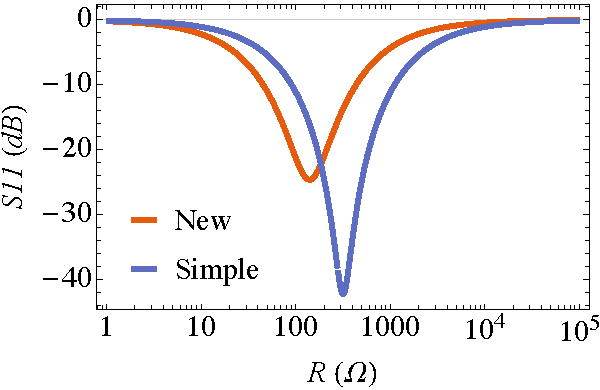
\includegraphics[width = 0.8\textwidth]{transfer_improved.pdf}
        \caption{Transfer function comparison between the model from Figure \ref{fig:improvedcircuit} and that in Figure \ref{fig:s11cs0db}.}
        \label{fig:improvedtransfer}
    \end{figure}

\end{frame}

\subsection{Optimisation}


\begin{frame}
    \frametitle{Optimisation using Shunt Capacitors}

    \begin{columns}
        \begin{column}{0.4\textwidth}
            \begin{itemize}
                \item One issue could be that the matching resistance is too low
                \item By adding a shunt capacitor in parallel, we should be able to shift the matching resistance
            \end{itemize}
        \end{column}
        \begin{column}{0.6\textwidth}

            \begin{figure}
                \centering
                \begin{circuitikz}[scale = 0.8] \draw
                    (0,0) to[short, o-] (0,-1) to[inductor, l_=$L:390\si{\nano\henry}$, -*] (0,-3)
                    (-1,-3) -- (1, -3) to[capacitor, l=$C_p:26\si{\pico\farad}$] (1, -5) -- (-1,-5) to[vR, l=$R$] (-1,-3)
                    (0, -5) to[short, *-] (0, -5.2) node[ground]{};
                    \draw[red]
                    (0,-0.5) to[short, *-] (1.5,-0.5) to[capacitor, l=$C_s$, color=red] (1.5,-2) node[ground, color=red]{}
                    ;
                \end{circuitikz}
                \caption{Circuit diagram for optimised RF reflectometry circuit.}
                \label{fig:opt_circuit}
            \end{figure}
            % \begin{figure}[tp]
            %     \centering
            %     \begin{tikzpicture}[x=0.75pt,y=0.75pt,yscale=-0.7,xscale=0.8]
            %         %uncomment if require: \path (0,368); %set diagram left start at 0, and has height of 368

            %         %Straight Lines [id:da06782621221887086] 
            %         \draw [line width=1.5]    (290,27.2) -- (290,80) ;
            %         %Straight Lines [id:da05438248126058465] 
            %         \draw [line width=1.5, color=red]    (380,60) -- (290,60) ;
            %         %Straight Lines [id:da158345526126636] 
            %         \draw [line width=1.5, color=red]    (380,60) -- (380,100) ;
            %         %Shape: Capacitor [id:dp8567246814632112] 
            %         \draw  [line width=1.5, color=red]  (380,100) -- (380,122.5) (400,127.5) -- (360,127.5) (400,122.5) -- (360,122.5) (380,127.5) -- (380,150) ;
            %         %Straight Lines [id:da7662482642077773] 
            %         \draw [line width=1.5]    (340,180) -- (242.5,180) ;
            %         %Shape: Resistor [id:dp8592626232820928] 
            %         \draw  [line width=1.5]  (250,194.4) -- (250,245.6) -- (234,245.6) -- (234,194.4) -- (250,194.4) -- cycle (242,180) -- (242,194.4) (242,245.6) -- (242,260) ;
            %         %Shape: Capacitor [id:dp2762209685239636] 
            %         \draw  [line width=1.5]  (340,190) -- (340,212.5) (360,217.5) -- (320,217.5) (360,212.5) -- (320,212.5) (340,217.5) -- (340,240) ;
            %         %Straight Lines [id:da6548911076200925] 
            %         \draw [line width=1.5]    (340,180) -- (340,190) ;
            %         %Straight Lines [id:da19597004940380347] 
            %         \draw [line width=1.5]    (340,240) -- (340,260) ;
            %         %Straight Lines [id:da8415802345776575] 
            %         \draw [line width=1.5]    (242,260) -- (340,260) ;
            %         %Shape: Ground [id:dp783868698411631] 
            %         \draw  [line width=1.5]  (276,271) -- (291,293) -- (306,271) -- (276,271) -- cycle (291,260) -- (291,271) ;
            %         %Shape: Ground [id:dp21245550286994108] 
            %         \draw  [line width=1.5, color=red]  (365,161) -- (380,183) -- (395,161) -- (365,161) -- cycle (380,150) -- (380,161) ;
            %         %Shape: Inductor (Air Core) [id:dp42625766752857785] 
            %         \draw  [line width=1.5]  (290,80) -- (290,94.9) .. controls (301.04,94.9) and (310,97.87) .. (310,101.53) .. controls (310,105.18) and (301.04,108.15) .. (290,108.15) .. controls (301.04,108.15) and (310,111.12) .. (310,114.78) .. controls (310,118.43) and (301.04,121.4) .. (290,121.4) .. controls (301.04,121.4) and (310,124.37) .. (310,128.02) .. controls (310,131.68) and (301.04,134.65) .. (290,134.65) .. controls (301.04,134.65) and (310,137.62) .. (310,141.27) .. controls (310,144.93) and (301.04,147.9) .. (290,147.9) -- (290,162.8) ;
            %         %Straight Lines [id:da061679490108252466] 
            %         \draw [line width=1.5]  (290,162.8) -- (290,180) ;

            %         % Text Node
            %         \draw (185,112) node [anchor=north west][inner sep=0.75pt]   [align=left] {L = 390 nH};
            %         % Text Node
            %         \draw (411,116) node [anchor=north west][inner sep=0.75pt, color=red]   [align=left] {Cs};
            %         % Text Node
            %         \draw (371,205) node [anchor=north west][inner sep=0.75pt]   [align=left] {Cp = 26 pF};
            %         % Text Node
            %         \draw (213,211) node [anchor=north west][inner sep=0.75pt]   [align=left] {R};

            %     \end{tikzpicture}
            % \caption{Circuit diagram for optimised RF reflectometry circuit.}
            % \label{fig:opt_circuit}
            % \end{figure}
        \end{column}
    \end{columns}


\end{frame}

\begin{frame}
    \frametitle{Simulations with Shunt Capacitors}

    The impedance of the new circuit (Figure \ref{fig:opt_circuit}) should be:

    \begin{equation}
        Z_t = \left[ \left(i\omega L + \frac1{\frac1R + i\omega C_p}\right)^{-1} + i\omega C_s \right]^{-1}
        \label{eq:zt}
    \end{equation}

    This can then be applied to Equation \ref{eq:s11} to simulate the effects of a shunt capacitor.

\end{frame}

\begin{frame}
    \frametitle{Simulations with Shunt Capacitors}

    \begin{columns}
        \begin{column}{0.5\textwidth}
            \begin{figure}
                \centering
                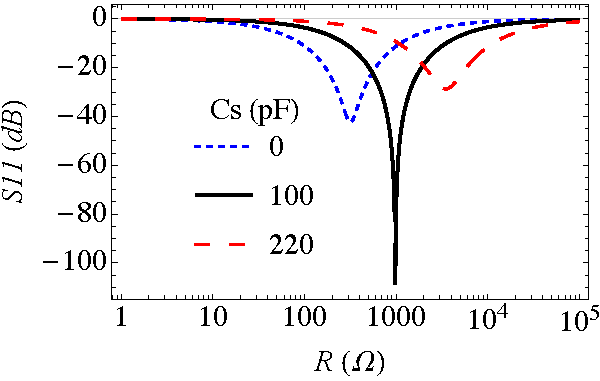
\includegraphics[width=\textwidth]{cs_comparison.pdf}
                \caption{Comparison of transfer functions with shunt capacitors.}
                \label{fig:cscomparison}
            \end{figure}
        \end{column}
        \begin{column}{0.5\textwidth}

            \begin{figure}
                \centering
                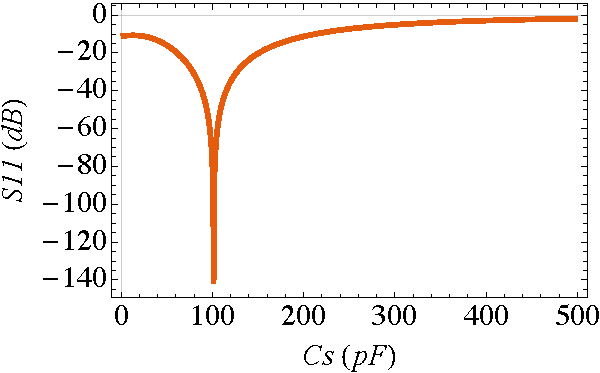
\includegraphics[width = \textwidth]{cs_simulation.pdf}
                \caption{Simulation of S11 values as a function of the included shunt capacitance, at a fixed value of $R = 1\si{\kilo\ohm}$.}
                \label{fig:cssimulation}
            \end{figure}
        \end{column}
    \end{columns}


\end{frame}

\begin{frame}
    \frametitle{RF Reflectometry With A Shunt Capacitor}

    \begin{columns}
        \begin{column}{0.5\textwidth}
            \begin{figure}
                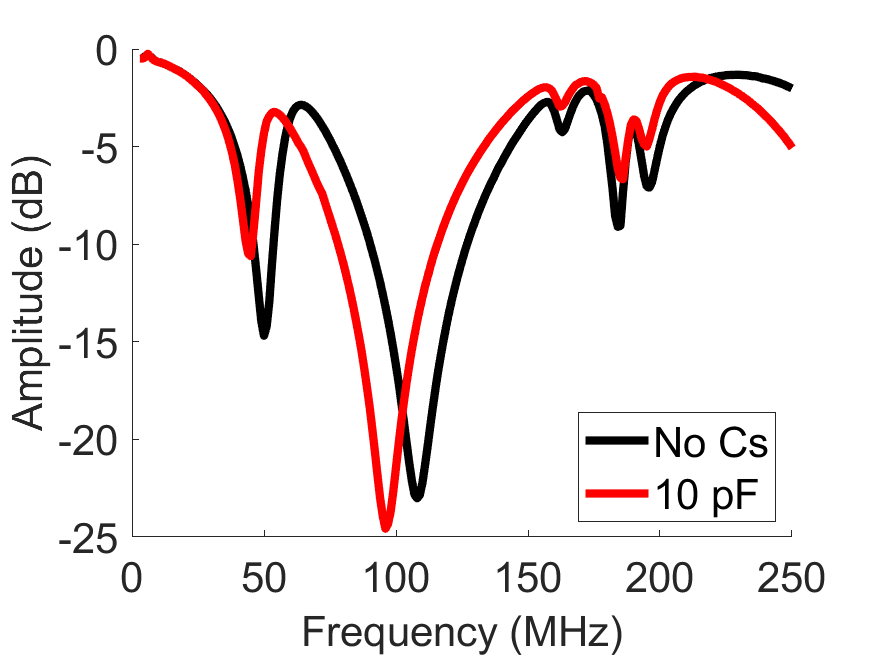
\includegraphics[width = 1.1\textwidth]{matlab_cs10_resonance.png}
                \caption{Resonance peaks with $C_s = 10\si{\pico\farad}$ and $C_s = 0$, holding $v_{DS} = -1\si{\volt}$, $v_\mathrm{gate}=0$.}
                \label{fig:cs10res}
            \end{figure}
        \end{column}
        \begin{column}{0.5\textwidth}
            \begin{figure}
                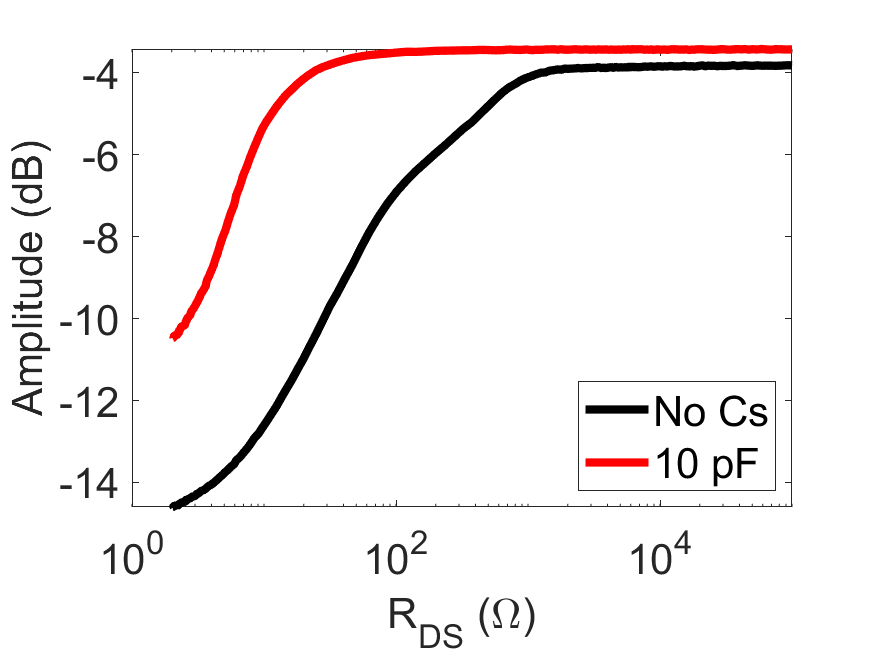
\includegraphics[width = 1.1\textwidth]{matlab_cs10_transfer.png}
                \caption{Transfer function at $f = 44\si{\mega\hertz}$ with $C_s = 10\si{\pico\farad}$ and at $f=50\si{\mega\hertz}$ with $C_s = 0$.}
                \label{fig:cs10transfer}
            \end{figure}
        \end{column}
    \end{columns}
\end{frame}

\begin{frame}
    \frametitle{RF Reflectometry With a Shunt Capacitor}

    %% At 1 MHz and 1 nF, the impedance of the shunt capacitor circuit is ~ Ohms;
    % therefore RF just goes through to ground; no resonance expected

    \begin{columns}
        \begin{column}{0.5\textwidth}
            \begin{itemize}
                \item When a $C_s = 220\si{\pico\farad}$ and a $C_s = 1\si{\nano\farad}$ capacitor were used, no resonance peaks were observed
            \end{itemize}
            This may be due to:
            \begin{itemize}
                \item At larger values of $C_s$, the impedance of the capacitor is lower than the RLC circuit
                \item This creates an RF path to ground, bypassing any resonance that may occur
            \end{itemize}
        \end{column}
        \begin{column}{0.5\textwidth}
            \begin{figure}
                \centering
                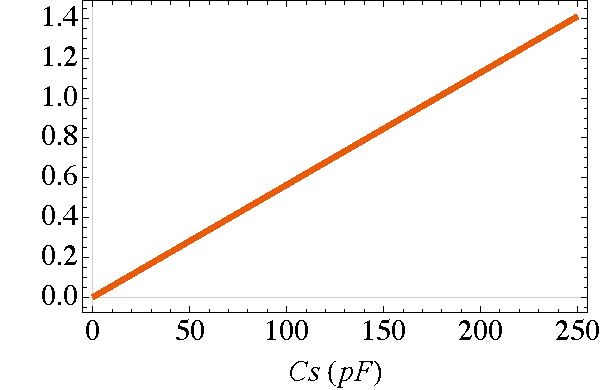
\includegraphics[width=\textwidth]{impedanceratio.pdf}
                \caption{Ratio of RLC impedance to $C_s$ impedance as a function of $C_s$, at $f=50\si{\mega\hertz}$.}
                \label{fig:impedanceratio}
            \end{figure}
        \end{column}
    \end{columns}

    %% We used commerical MOSFET to characterise the board; 
    % Figured out about capacitors required, setting up and operating
    % But the MOSFET is not a perfect simulation; has a large Cp (literature often has Cp ~ 1pF)
    % Therefore would be beneficial to use a more realistic device 

\end{frame}

\section{Subprojects}

\subsection{Variable Capacitors}

\begin{frame}
    \frametitle{Variable Capacitors}

    %% fix this

    \begin{itemize}
        \item Attempted to incorporate a variable shunt capacitor onto the CPH daughter board with the transistor
        \item Also attempted with a new silicon MOSFET device with smaller $C_p$ and larger $R$
        \item However was unable to measure the effective capacitance and resonance due to equipment difficulties
    \end{itemize}

\end{frame}

\begin{frame}
    \frametitle{Future Directions}

    \begin{itemize}
        \item Beneficial to compare impedances on a device known to respond to shunt capacitances
        \item Repeat methods with a $100\si{\nano\farad}$ capacitor (the theoretical optimum)
    \end{itemize}

\end{frame}

\subsection{BB4}

\begin{frame}
    \frametitle{$4\si{\kelvin}$ Testing of Germanium Quantum Dot}

    \begin{columns}
        \begin{column}{0.3\textwidth}
            Gate tested $BB4$ (germanium quantum dot) at $4\si{\kelvin}$ to check that all the gates and ohmics work correctly.
        \end{column}
        \begin{column}{0.7\textwidth}
            \begin{figure}
                \centering
                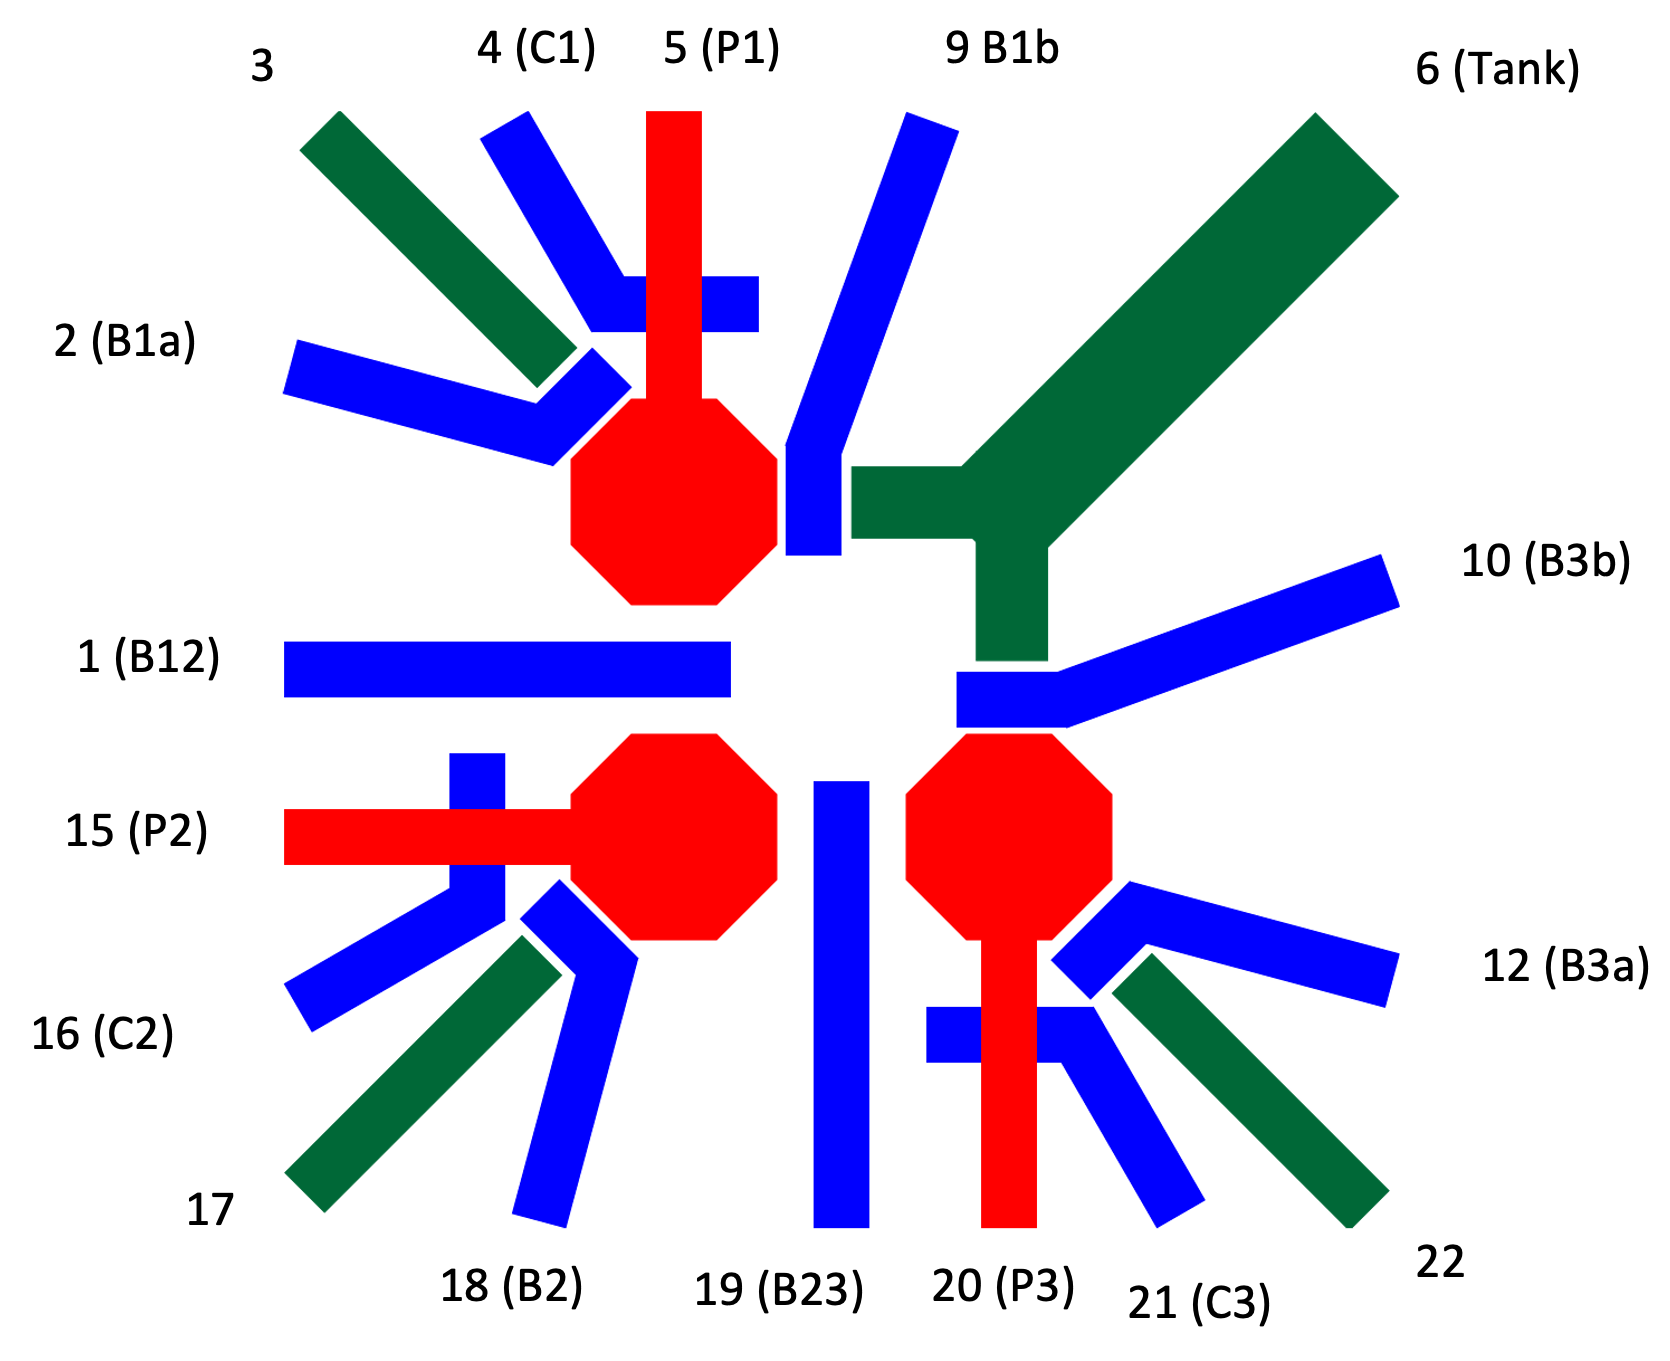
\includegraphics[width=0.8\textwidth]{bb4.png}
                \caption{Schematic diagram of the gates on the device; green - ohmics; blue - barrier electrodes; red - plunger electrodes}
            \end{figure}
        \end{column}
    \end{columns}


\end{frame}

\subsection{Other}

\begin{frame}
    \frametitle{Other Subprojects}

    \begin{itemize}
        \item Tested all contacts on two CPH boards
        \item Updated AWG Pulse Studio for MATLAB v2 and implemented a parametric function option
        \item Updated VNA driver for MATLAB v2
        \item Created a driver for the Keithley SM2401 source meter in MATLAB v2
        \item Created a driver for the Yokogawa IM7651 Variable DC Source in MATLAB v2
    \end{itemize}

\end{frame}

\begin{frame}
    \frametitle{ }
    \begin{center}
        Thank you!
    \end{center}

\end{frame}

\begin{frame}
    \frametitle{Appendix}

    \begin{figure}
        \centering
        \begin{circuitikz}[scale = 0.8]
            \draw
            (0,0) to[short, o-, i =$~$] (1,0) to[capacitor, l=$C_{BT}$] (2,0)
            to[capacitor, l=$C_9$] (3,0) to[capacitor, l=$C_6$] (4,0) -- (5,0)
            to[inductor, l=$L_4$] (6,0) -- (7,0) to[vR, l=$R$] (8,0) -- (9,0)
            to[capacitor, l=$C_{LF}$] (10,0) -- (10.5, 0) node[ground]{}
            (4.5, 0) to[short, *-] (4.5, -3) to[C, l_=$C_s$] ++(1,0) to[C, l_=$C_7$] ++(1,0) -- ++(0.5,0) node[ground]{}
            (6.5, 0) to[short, *-] (6.5, -1.5) to[C, l_=$C_p$] (7.5, -1.5) -- (8, -1.5) node[ground]{}
            ;
        \end{circuitikz}
        \caption{Figure \ref{fig:improvedcircuit} with added shunt capacitor.}
        \label{fig:improvedcircuitshunt}
    \end{figure}

\end{frame}

\begin{frame}
    \frametitle{Appendix}

    \begin{figure}
        \centering
        \begin{circuitikz}[scale = 0.8]
            \draw
            (0,0) to[short, o-, i = $I_{DS}$] ++(1,0) to[R, l=$R_{LF}$] ++(2,0) to[R, l=$R_{TC}$] ++(2,0) to[inductor, l=$L_4$] ++(2,0) -- ++(0.5,0)
            ++(0.8, 0) node[npn, rotate=-90, yscale=-1]{}
            ++(0.8,0) -- ++(0.4,0) to[R, l=$R_{LF}$] ++(2,0) to[short, -o] ++(1,0)
            ;
        \end{circuitikz}
        \caption{DC circuit supplying the transistor.}
        \label{fig:dccircuit}
    \end{figure}

\end{frame}

\begin{frame}
    \frametitle{Appendix}

    \begin{figure}
        \centering
        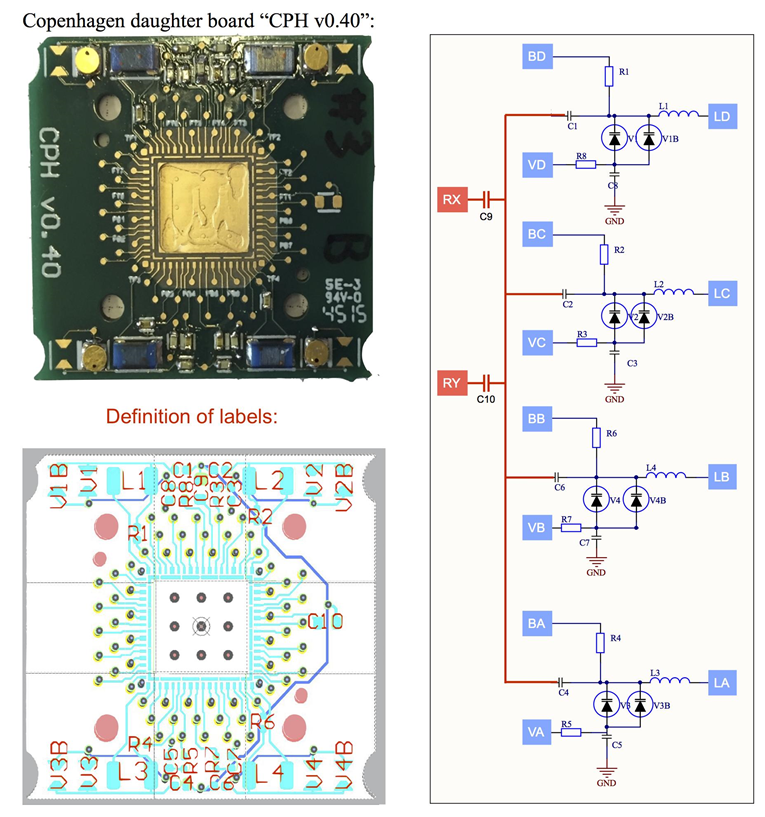
\includegraphics[height=0.8\textheight]{cph_schematic.png}
    \end{figure}

\end{frame}

\begin{frame}
    \frametitle{Resonance Maps}

    \begin{columns}
        \begin{column}{0.5\textwidth}
            \begin{figure}
                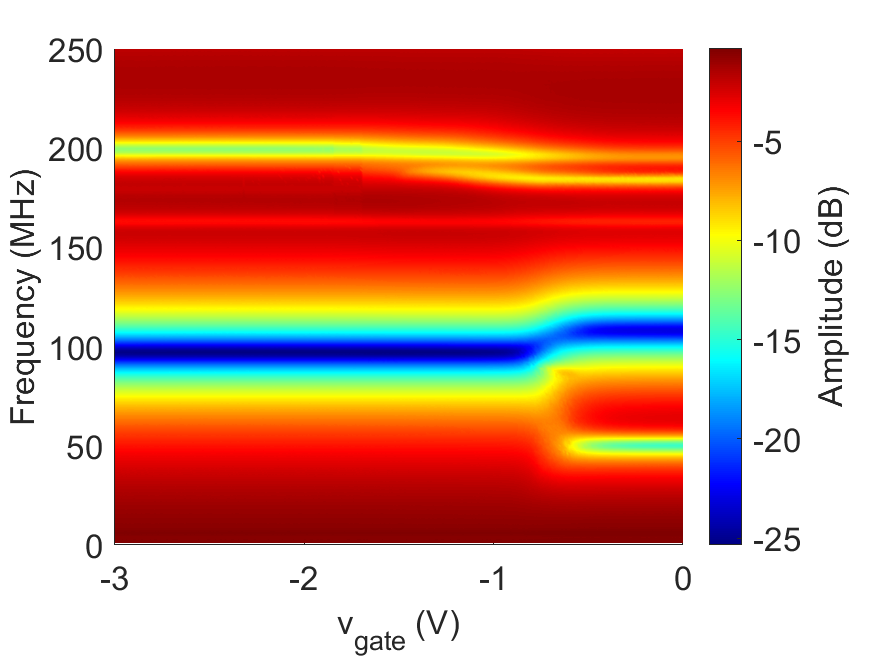
\includegraphics[width = 1.1\textwidth]{2102xxrf_001_2021.02.02.17.34.26_final_rf-surf.png}
                \caption{Resonance peaks at various $v_\mathrm{gate}$, without a shunt capacitor.}
            \end{figure}
        \end{column}
        \begin{column}{0.5\textwidth}
            \begin{figure}
                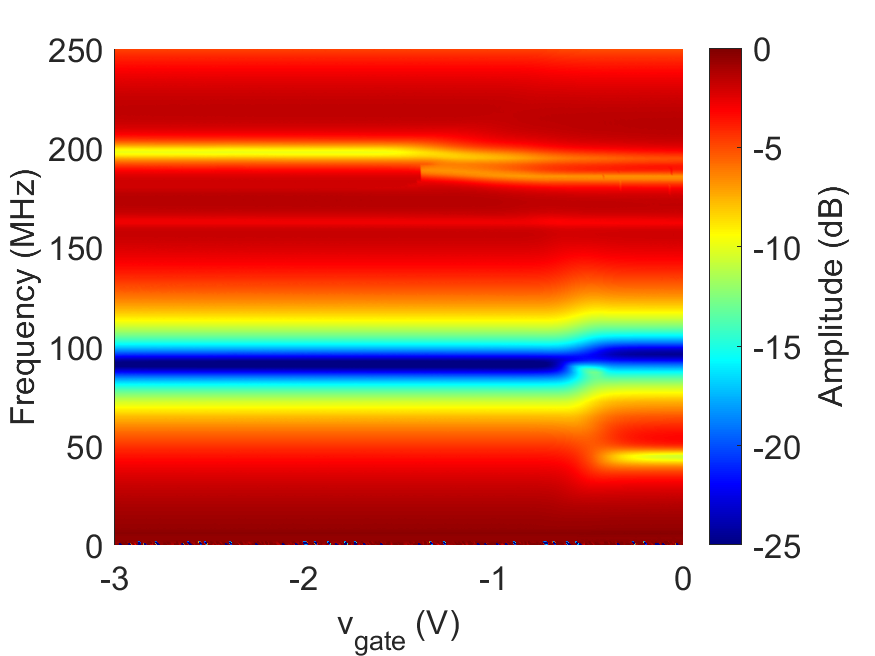
\includegraphics[width = 1.1\textwidth]{210212rf_003_2021.02.12.12.49.25_final_rf.png}
                \caption{Resonance peaks at various $v_\mathrm{gate}$, with $C_s = 10\si{\pico\farad}$.}
            \end{figure}
        \end{column}
    \end{columns}

\end{frame}

\begin{frame}
    \frametitle{Transfer Functions}

    \begin{columns}
        \begin{column}{0.5\textwidth}
            \begin{figure}
                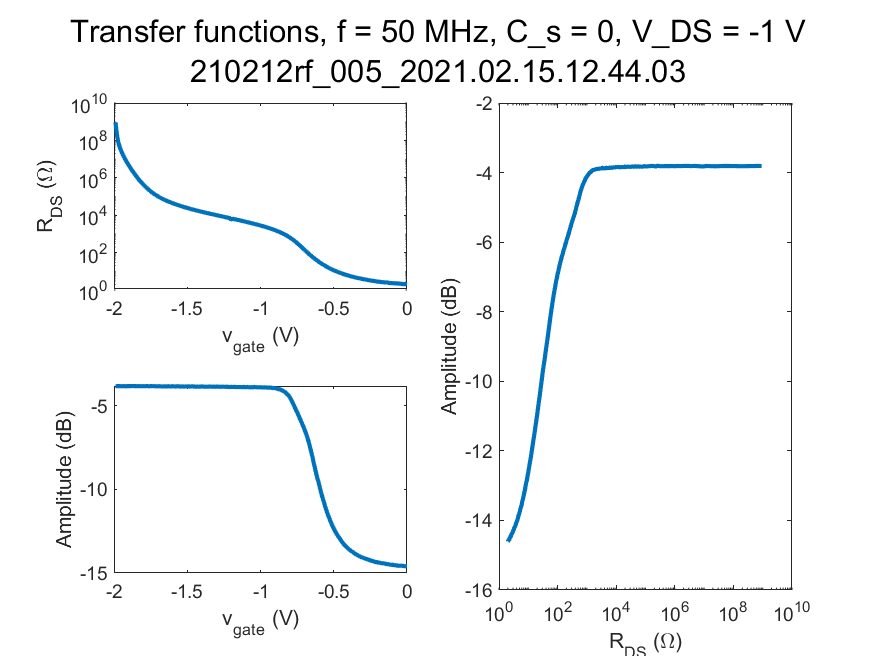
\includegraphics[width = 1.1\textwidth]{210212rf_005_2021.02.15.12.44.03_final_rf-transfer.png}
                \caption{Transfer function at $f = 50\si{\mega\hertz}$ and $v_{DS} = -1\si{\volt}$, with no shunt capacitor}
            \end{figure}
        \end{column}
        \begin{column}{0.5\textwidth}
            \begin{figure}
                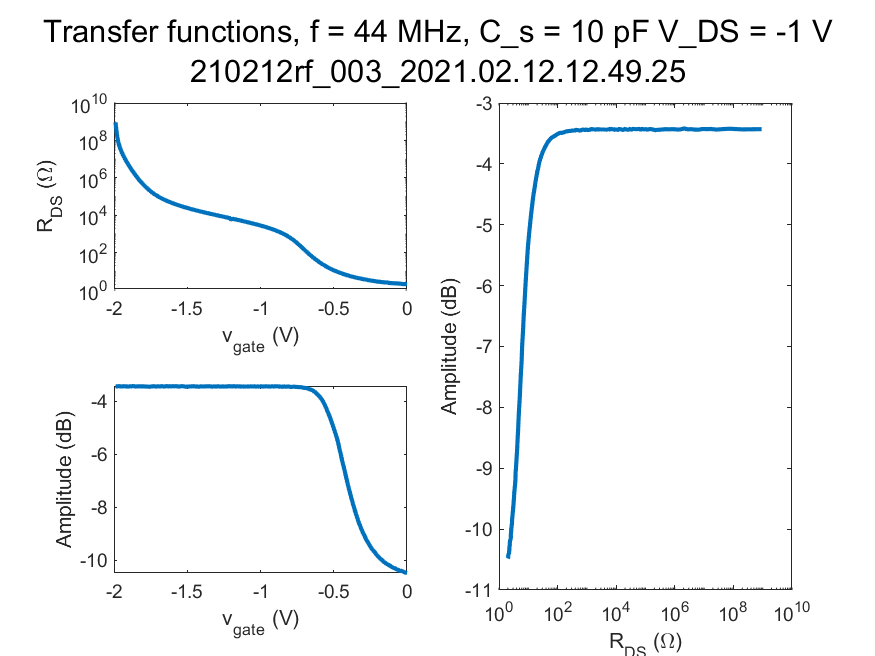
\includegraphics[width = 1.1\textwidth]{210212rf_003_2021.02.12.12.49.25_final_rf-transfer.png}
                \caption{Transfer function at $f = 44\si{\mega\hertz}$, with $C_s = 10\si{\pico\farad}$.}
            \end{figure}
        \end{column}
    \end{columns}

\end{frame}

\end{document}